%% Creator: Inkscape 1.3.2 (091e20ef0f, 2023-11-25), www.inkscape.org
%% PDF/EPS/PS + LaTeX output extension by Johan Engelen, 2010
%% Accompanies image file 'wpol_g152.pdf' (pdf, eps, ps)
%%
%% To include the image in your LaTeX document, write
%%   \input{<filename>.pdf_tex}
%%  instead of
%%   \includegraphics{<filename>.pdf}
%% To scale the image, write
%%   \def\svgwidth{<desired width>}
%%   \input{<filename>.pdf_tex}
%%  instead of
%%   \includegraphics[width=<desired width>]{<filename>.pdf}
%%
%% Images with a different path to the parent latex file can
%% be accessed with the `import' package (which may need to be
%% installed) using
%%   \usepackage{import}
%% in the preamble, and then including the image with
%%   \import{<path to file>}{<filename>.pdf_tex}
%% Alternatively, one can specify
%%   \graphicspath{{<path to file>/}}
%% 
%% For more information, please see info/svg-inkscape on CTAN:
%%   http://tug.ctan.org/tex-archive/info/svg-inkscape
%%
\begingroup%
  \makeatletter%
  \providecommand\color[2][]{%
    \errmessage{(Inkscape) Color is used for the text in Inkscape, but the package 'color.sty' is not loaded}%
    \renewcommand\color[2][]{}%
  }%
  \providecommand\transparent[1]{%
    \errmessage{(Inkscape) Transparency is used (non-zero) for the text in Inkscape, but the package 'transparent.sty' is not loaded}%
    \renewcommand\transparent[1]{}%
  }%
  \providecommand\rotatebox[2]{#2}%
  \newcommand*\fsize{\dimexpr\f@size pt\relax}%
  \newcommand*\lineheight[1]{\fontsize{\fsize}{#1\fsize}\selectfont}%
  \ifx\svgwidth\undefined%
    \setlength{\unitlength}{352.12479238bp}%
    \ifx\svgscale\undefined%
      \relax%
    \else%
      \setlength{\unitlength}{\unitlength * \real{\svgscale}}%
    \fi%
  \else%
    \setlength{\unitlength}{\svgwidth}%
  \fi%
  \global\let\svgwidth\undefined%
  \global\let\svgscale\undefined%
  \makeatother%
\begin{textblock}{1}(0,0)
  \begin{picture}(1,0.96503218)%
\only<1->{
    \lineheight{1}%
    \setlength\tabcolsep{0pt}%
    \put(0,0){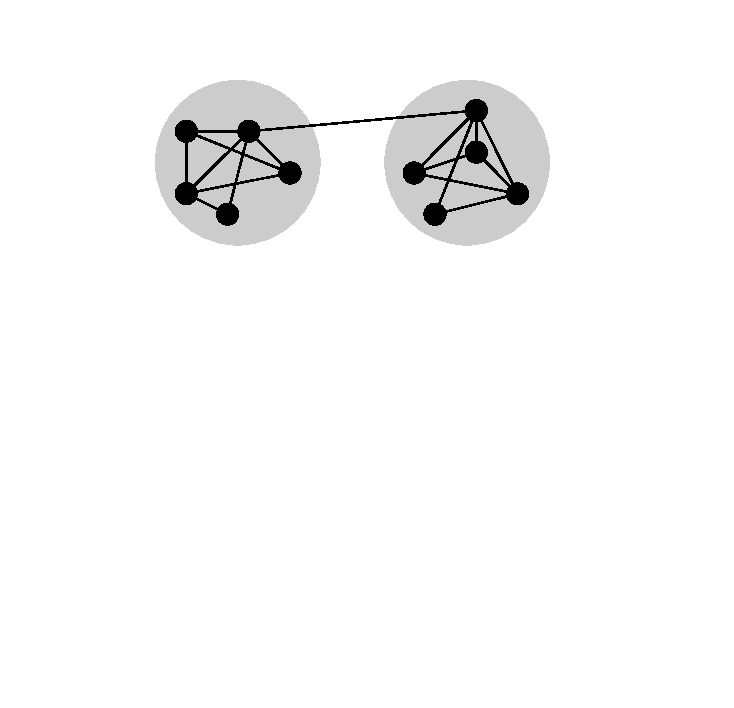
\includegraphics[width=\unitlength,page=1]{wpol_g152.pdf}}%
}
\only<4->{
    \lineheight{1}%
    \setlength\tabcolsep{0pt}%
    \put(0.47951581,0.80753644){\color[rgb]{0,0,0}\makebox(0,0)[t]{\lineheight{1.25}\smash{\begin{tabular}[t]{c}$2$\end{tabular}}}}%
    \put(0.30099468,0.79322597){\color[rgb]{0,0,0}\makebox(0,0)[t]{\lineheight{1.25}\smash{\begin{tabular}[t]{c}$7$\end{tabular}}}}%
    \put(0.242498,0.73850161){\color[rgb]{0,0,0}\makebox(0,0)[t]{\lineheight{1.25}\smash{\begin{tabular}[t]{c}$8$\end{tabular}}}}%
    \put(0.27309547,0.66684179){\color[rgb]{0,0,0}\makebox(0,0)[t]{\lineheight{1.25}\smash{\begin{tabular}[t]{c}$9$\end{tabular}}}}%
    \put(0.28033205,0.74224816){\color[rgb]{0,0,0}\makebox(0,0)[t]{\lineheight{1.25}\smash{\begin{tabular}[t]{c}$10$\end{tabular}}}}%
    \put(0.34671701,0.72698518){\color[rgb]{0,0,0}\makebox(0,0)[t]{\lineheight{1.25}\smash{\begin{tabular}[t]{c}$8$\end{tabular}}}}%
    \put(0.32795795,0.69257023){\color[rgb]{0,0,0}\makebox(0,0)[t]{\lineheight{1.25}\smash{\begin{tabular}[t]{c}$5$\end{tabular}}}}%
    \put(0.31412802,0.72452411){\color[rgb]{0,0,0}\makebox(0,0)[t]{\lineheight{1.25}\smash{\begin{tabular}[t]{c}$6$\end{tabular}}}}%
    \put(0.37361678,0.76132298){\color[rgb]{0,0,0}\makebox(0,0)[t]{\lineheight{1.25}\smash{\begin{tabular}[t]{c}$7$\end{tabular}}}}%
    \put(0.6031723,0.77559584){\color[rgb]{0,0,0}\makebox(0,0)[t]{\lineheight{1.25}\smash{\begin{tabular}[t]{c}$9$\end{tabular}}}}%
    \put(0.60838026,0.74871008){\color[rgb]{0,0,0}\makebox(0,0)[t]{\lineheight{1.25}\smash{\begin{tabular}[t]{c}$6$\end{tabular}}}}%
    \put(0.59296176,0.69951535){\color[rgb]{0,0,0}\makebox(0,0)[t]{\lineheight{1.25}\smash{\begin{tabular}[t]{c}$2$\end{tabular}}}}%
    \put(0.66412206,0.71786745){\color[rgb]{0,0,0}\makebox(0,0)[t]{\lineheight{1.25}\smash{\begin{tabular}[t]{c}$9$\end{tabular}}}}%
    \put(0.69057827,0.75346103){\color[rgb]{0,0,0}\makebox(0,0)[t]{\lineheight{1.25}\smash{\begin{tabular}[t]{c}$8$\end{tabular}}}}%
    \put(0.6557511,0.77630927){\color[rgb]{0,0,0}\makebox(0,0)[t]{\lineheight{1.25}\smash{\begin{tabular}[t]{c}$1$\end{tabular}}}}%
    \put(0.65242202,0.66629179){\color[rgb]{0,0,0}\makebox(0,0)[t]{\lineheight{1.25}\smash{\begin{tabular}[t]{c}$10$\end{tabular}}}}%
    \put(0.63658085,0.69284231){\color[rgb]{0,0,0}\makebox(0,0)[t]{\lineheight{1.25}\smash{\begin{tabular}[t]{c}$7$\end{tabular}}}}%
}
  \end{picture}%
  \end{textblock}
\endgroup%
